%!TEX root = ../template.tex

\chapter{Approach to Elaboration Phase}
\label{cha:approach_to_elaboration_phase}

This chapter will discuss and present an overview of the elaboration phase. It will describe in fine detail the objective and contributions of this dissertation and how it is planned to archive those goals. It should provide a detailed and clear roadmap to implement a system that will comply with all the objectives goals and requirements of this thesis.

In section \ref{sec:refinement_of_objectives_and_contributions} the objectives and contributions are refined and exposed clearly and matched against the related work performed and discussed in chapter \ref{cha:related_work}. It will discuss the scenario and environment under where the system should fall.

Section \ref{sec:system_model_approach} its presented the general system model of the contributions and objectives. It describes the model of the planned system implementation.

The architecture and implementation details of the solution are present in section \ref{sec:planned_architecture_and_implementation}. This section will dive in more detail on how and with what technologies the system will be implemented with.

Having discussed the solution implementation, section \ref{sec:planned_testbench_environments} explains how and where it is planned to test the system, whereas section \ref{sec:relevant_evaluation_criteria} will complement it with what metrics will be gathered and how they will be compared with each other.

\section{Refinement of Objectives and Contributions} % (fold)
\label{sec:refinement_of_objectives_and_contributions}

To achieve the objectives proposed in chapter \ref{cha:introduction}, we will work under a specific scenario, that can be described using an adversary model and some system assumptions. The goal of creating a secure in-memory storage based on secure hardware technologies must have a well defined scope and be thorough across that same scope. The system adversary/threat model and assumptions will be described in sections \ref{ssec:adversary_model} and \ref{ssec:system_assumptions} respectively.

\subsection{Adversary Model}
\label{ssec:adversary_model}

The threat model basis for the system will lie on the gls{SGX}'s model. We will assume their model and protection overview stated in \gls{SGX}'s paper \cite{sgx:7}.

\textit{SGX prevents all other software from accessing the code and data located inside an enclave including system software and access from other enclaves. Attempts to modify an enclave’s contents are detected and either prevented or execution is aborted}, \cite{sgx:7} which falls in the following adversary model:

\textbf{Malicious applications or code:} The system protects its data from an attacker capable of compromising the system through another application installed on the same system. This includes code from the \gls{OS} hypervisor or any other code in the machine.

\textbf{Honest but Curious (or Malicious System Administrator):} The system must be able to protect from an attacker with root access to the machine. Data deployed on the cloud should only be read by the user and not by any cloud system administrators with ability to examine and modify the system.

\textbf{Network Attacks:} All communication to and from the system should be secure. We assume attacker capable of intercepting, replaying and tamper with messages in the transport layer. 

\textbf{File system and memory access attacks:} All sensitive data residing outside protected memory should be encrypted. An attacker can access the physical disks and hardware without the data being exposed.

\subsection{System Assumptions}
\label{ssec:system_assumptions}

The system planned has certain assumptions and aspects that are considered to be out of scope for this dissertation:

\begin{itemize}
	\item \textbf{Trusted Client} - The client side is assumed to be completely trusted and correct.
	\item \textbf{\gls{DoS} and \gls{DDoS}} attacks are out of scope.
	\item \textbf{Side Channel Attacks} - It is out of scope any side channel attacks or any related attack not present in \gls{SGX}'s threat model.
	\item \textbf{Physical and Hardware attacks} - It is out of scope any physical or hardware attacks or any related attack not present in the \gls{SGX} threat model.
	\item \textbf{\gls{SGX} limitations or security issues} - Any limitation or security issues known to the technology, either present on the \gls{SGX}'s paper and/or explain in section \ref{ssec:circumvention_of_sgx_limitations}.
	\item \textbf{Bizantine Fault Tolerance} - It is out of scope to tolerate a bizantine fault tolerance model
\end{itemize}

\section{System Model Approach} % (fold)
\label{sec:system_model_approach}

The main goal of this project is modelled in figure \ref{fig:syste_model_detailed}. As shown, the model can be divided in three main components - the \textbf{client} which was already defined as out of scope, the \textbf{communications} and the \textbf{backend service}. 

\begin{figure}[htbp]
  \centering{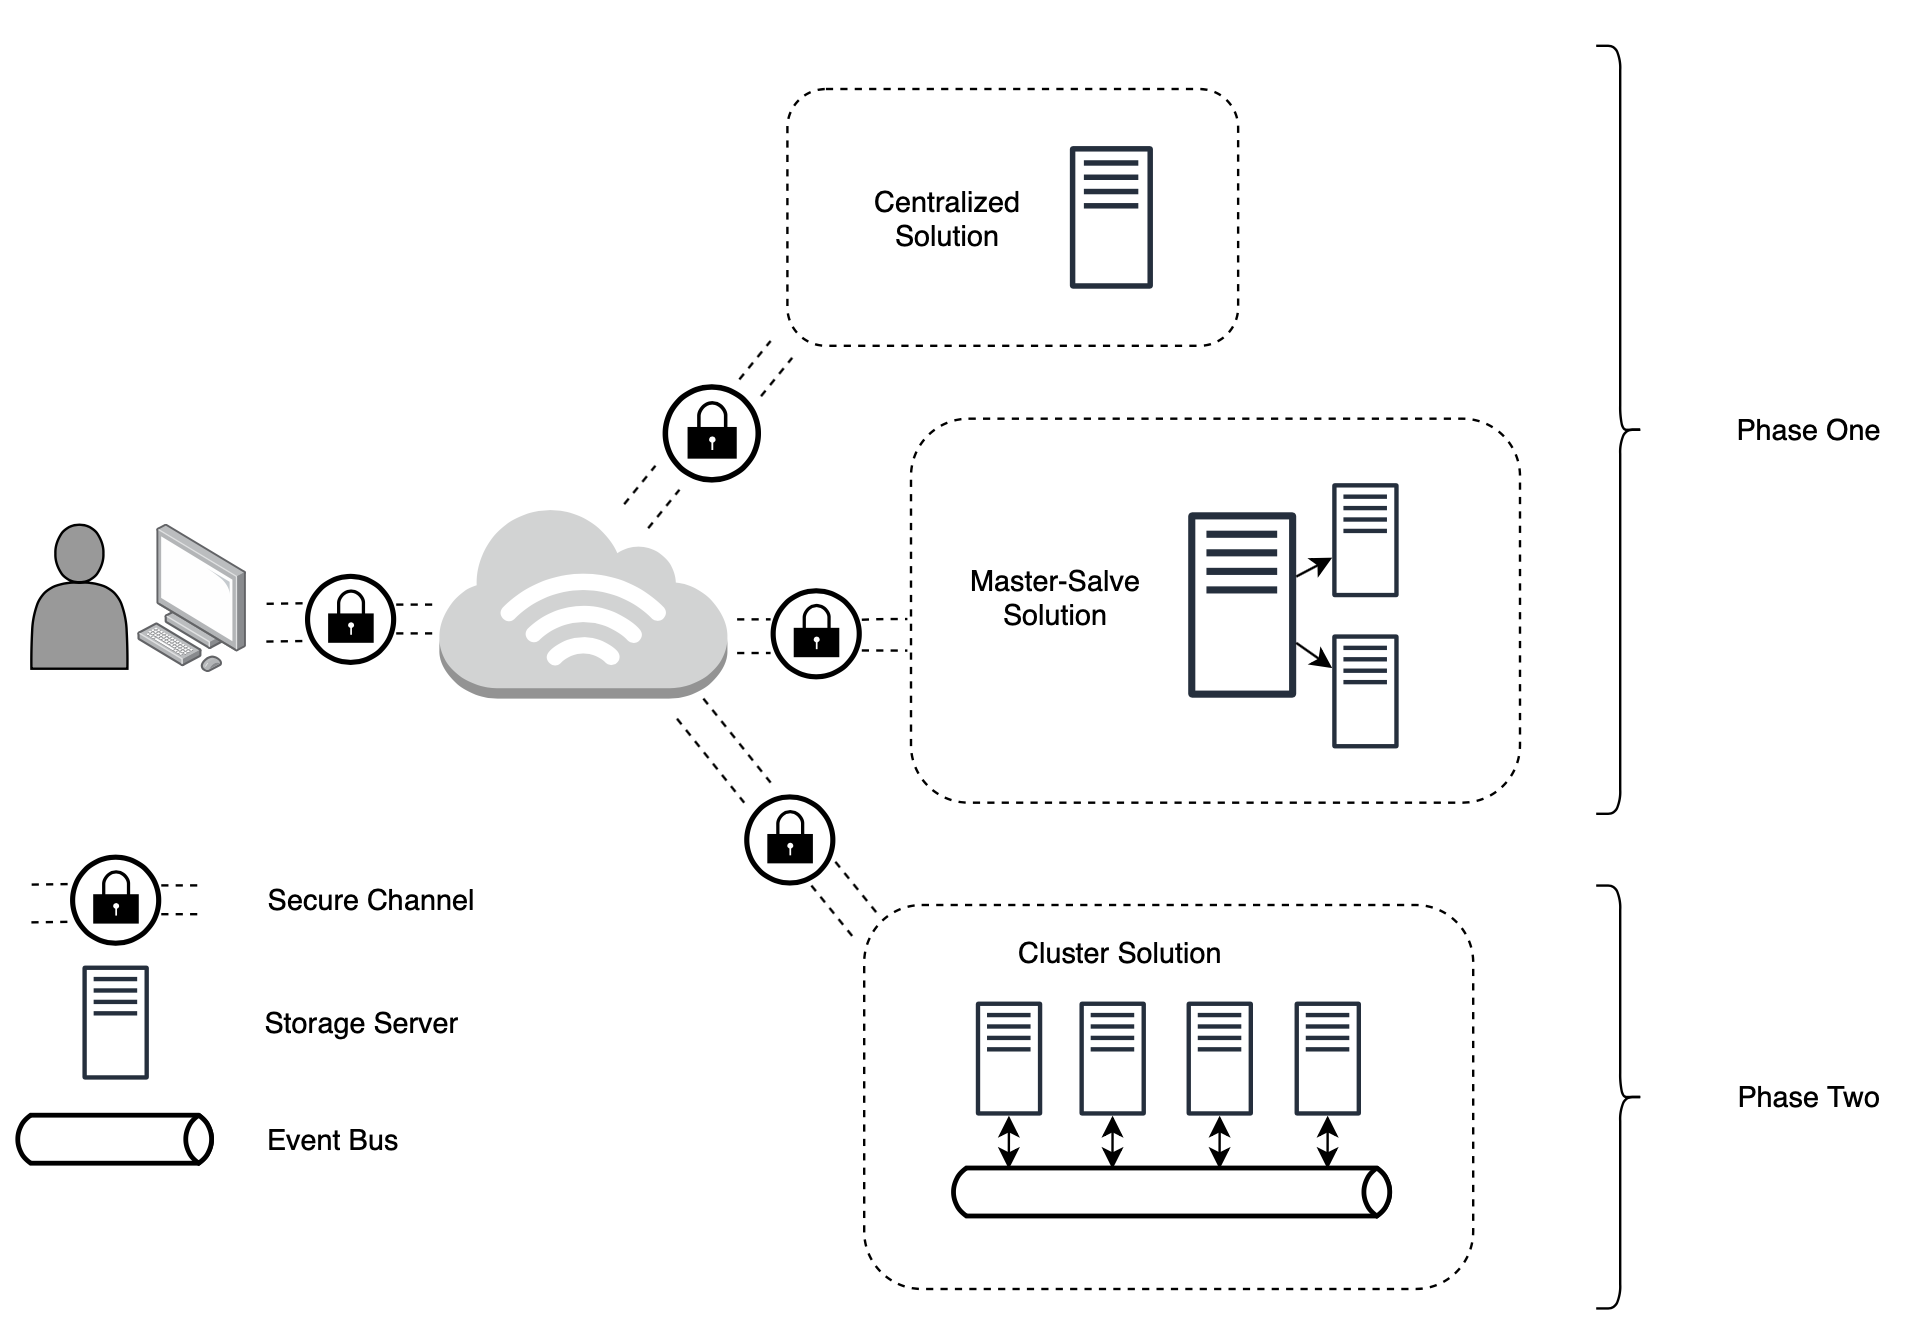
\includegraphics[width=0.9\linewidth]{SystemModelDetailed}}%
  \caption{System Model Details}
  \label{fig:syste_model_detailed}
\end{figure}

The main focus of this project is the backend service which will be divided in two phases. Phase One will envolve two different types of replication (no replication and Master-Slave solution) and phase two, will implement another, although a more complex one, replication algorithm called the cluster solution.

The system should comply with the adversary and threat model explained in section \ref{ssec:adversary_model}. The user should not be aware and should have seamless interaction with the system despiste the implementation provided by the backend, meaning that all solution should provide the same \gls{API} and support an interface as equal as possible to the unprotected version of the Key-Value Store.

\section{Planned Architecture and Implementation} % (fold)
\label{sec:planned_architecture_and_implementation}

Cloud providers these days offer their services and applications in different stacks and computing infrastructures. They can be categorised in three main and most common: \gls{IaaS} (Infrastructure as a Service), \gls{PaaS} (Platform as a Service), and \gls{SaaS} (Software as a Service). These are terms to represent how much of the stack is available for user customisation and how much is managed by the cloud provider. Figure \ref{fig:computing_stacks} shows the two stacks that were a possibility for the deployment of this service where the shaded components represent the ones managed by the provider.

\begin{figure}[htbp]
  \centering
  \subcaptionbox{IaaS Stack\label{fig:iaas_stack}}%
    {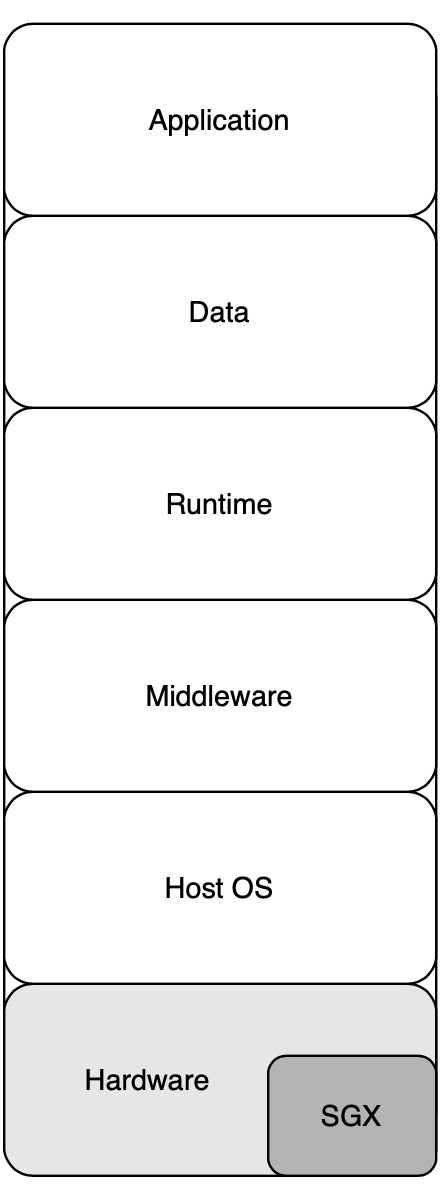
\includegraphics[width=0.2\linewidth]{IaaS_stack}}%
    \hspace{5em}
  \subcaptionbox{PaaS Stack\label{fig:paas_stack}}%
    {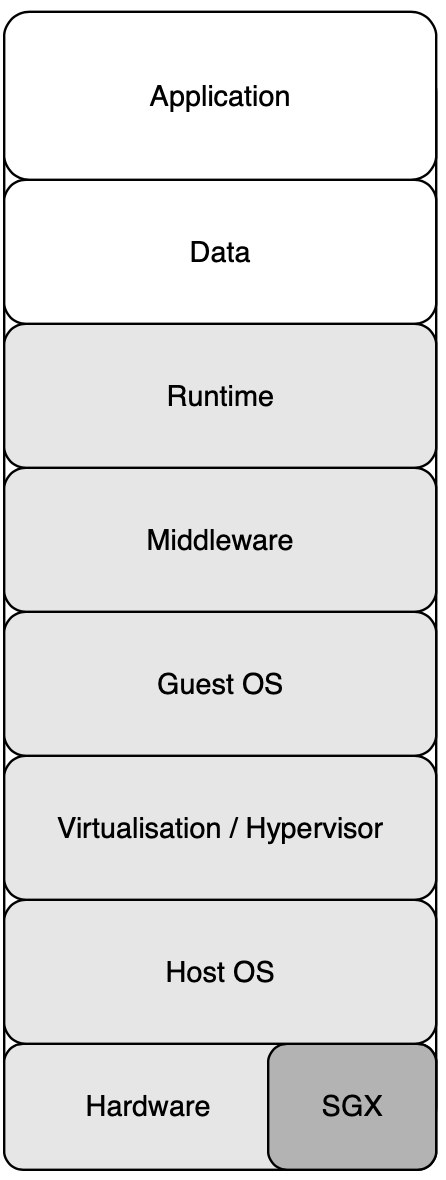
\includegraphics[width=0.2\linewidth]{PaaS_stack}}%
  \caption{Computing Stacks}
  \label{fig:computing_stacks}
\end{figure}

Figure \ref{fig:iaas_stack} is the stack chosen because it is the simpler to customise and change to our needs especially for development. Everything besides the physical hardware can be customisable and it is managed by the user. As for figure \ref{fig:paas_stack} it provides to the user a more abstracted environment, requiring less knowledge of computing bases and setups. Although, the offering of \glspl{PaaS} with the software needed for this project is very limited and the lack of customisation would work against the effort that the development phase will need \cite{computing_stacks:1}.

As shown on figure \ref{fig:computing_stacks} and to achieve the objectives and goals of the project (\ref{sec:objectives_and_planned_contributions}), the hardware chosen was Intel's \gls{SGX} secure module. As explained in section \ref{ssec:intel_sgx}, this technology has the means and the reach to provide a truly isolated environment has required in this dissertation. The stack will be running a Linux Ubuntu Server \cite{ubuntu_server:1} operating system as the Host \gls{OS}, version 18.04 LTS. this version has compatibility with Intel's \gls{SGX} hardware and with some software needed in another layer of the stack.

For the reasons explained in section \ref{ssec:redis}, Redis will be the key-value store application that will be worked on. This is the most used and most known \gls{KVS} technology, written in C language and will be deployed on the application component of the stack. To make Redis a trusted in-memory store, three main and crtitical components were identified and are candidates to run in an isolated environment inside the \gls{SGX}'s secure enclave (\ref{ssec:intel_sgx}):

\begin{itemize}
	\item Authentication and Access Control
	\item Memory Read/Write Operations
	\item Encryption/Decryption Mechanisms
\end{itemize}

The result of these critical components running inside an enclave, is the data stored in memory will be encrypted thus not available to the public eye (i.e: Cloud providers system administrators), and the flow of encrypting this data and storing this data will be performed isolated from any external attacker, therefore achieving several objectives proposed for this dissertation.

To help with \gls{SGX} integration a middleware software called Graphene \cite{graphene:1} will be used. This technology is a library \gls{OS} that \textit{"with \gls{SGX} support (...) can secure a critical application in a hardware-encrypted memory region. Graphene can protect applications from a malicious system stack with minimal porting effort"}. This library has already been tested with Linux Ubuntu Server 18.04 running as the \gls{OS}.

Communications will be secure with the help of SGXStunnel \cite{sgxstunnel:1}, a prototype proxy to support TLS tunnelling with endpoints executed in a trusted execution environment provided by Intel SGX. \gls{SGX} termination means that the packets will be decrypted inside the secure module, which allows the network drivers, modules and physical cards to be removed from the \gls{TCB}.

The solution for phase one (centralised and master-slave) will be implemented using the built-in mechanisms provided by Redis itself. Phase 2 will make use of an external module that provides clustering capabilities using an event bus. Kafka \cite{kafka:1} is the technology use to disseminate events across all Redis instances. The security of the event bus will be critical and all event transmitted should be encrypted.

\section{Planned Testbench Environments} % (fold)
\label{sec:planned_testbench_environments}

The services will be deployed and tested in two different environments. The first one will be called the \textbf{development environment}, which translates to a local virtual machine that aims to simulate and be as close as possible to the production environment, with the ease of development and rapid deployments. The \textbf{production environment} will be a deployment of the services on a cloud provider that offers \gls{SGX} dedicated hardware, like OVHcloud \cite{ovhcloud:1}.

The tests will pe performed by a combination of the built-in Redis-Client benchmark tests \cite{redis_benchmark_cli:1} and to eliminate any bias claims, an external tester like the Yahoo! Cloud Serving Benchmark \cite{yahoo_benchmark:1}.

\section{Relevant Evaluation Criteria} % (fold)
\label{sec:relevant_evaluation_criteria}

The testers and benchmark clients will evaluate metrics that can be compared with a non secure solution on the network side as well as the server side. On the network, latency, throughput, and operations per seconds (ops/s) and on the server side it will monitor the resources of the machines, like memory consumption and CPU load during the performance tests. It will also monitor and evaluate the concurrency problems that can be introduced by the replication mechanisms, like data loss, dirty reads and the time for the system to achieve a correct state among all replicas.
